\documentclass[12pt, twoside, a4paper]{article}

%pdfTeX
% \usepackage[utf8]{inputenc}
% \usepackage[T1]{fontenc}


\usepackage[margin=1truein]{geometry}
% \usepackage[T2A]{fontenc}
\usepackage[utf8]{inputenc}
\usepackage[english, russian]{babel}
% \usepackage[serbian]{babel}
% \usepackage[utf8]{fontenc}
% \usepackage[english,serbian]{babel}
% \usepackage[bitstream-charter]{mathdesign}

% \usepackage{palatino}
% \usepackage{charter}
% \usepackage{lmodern}

\usepackage{amsmath}
\usepackage{amssymb}
\usepackage{graphicx}
\usepackage[figurename=Slika,labelfont=bf]{caption}
\usepackage{tabularx}
\usepackage{mathtools}
\usepackage{pdflscape}
\usepackage{rotating}
\usepackage{enumitem}
\usepackage{bclogo}
% \usepackage{fontawesome}

% \usepackage[symbol]{footmisc}

%\usepackage{imakeidx}
\usepackage[xindy]{imakeidx}

\makeindex[columns=2, title=Индекс]

\renewcommand\indexname{Индекс}
\addto\captionsrussian{\renewcommand{\indexname}{Индекс}}

\indexsetup{        % if unspecified, "level" defaults to \chapter* or \section*
%level=\chapter      % numbered chapter in book class
level=\section     % numbered section in article class
}

\def\idx#1{#1\index{#1}}

\usepackage[dvipsnames]{xcolor}

\definecolor{darkblue}{rgb}{0, 0, 0.4}
\usepackage[
  colorlinks = true,
  urlcolor = darkblue,
  linkcolor = black
]{hyperref}

\usepackage{qrcode}
\usepackage{svg}
\usepackage{wrapfig}

\usepackage{totcount}
\newtotcounter{zadaci}
\setcounter{zadaci}{0}

\input serbian


\DeclareGraphicsRule{*}{mps}{*}{}

\renewcommand*\contentsname{Sadr{\zv}aj}
\addto\captionsrussian{\renewcommand{\contentsname}{Садржај}}

\usepackage{titlesec}
\newcommand{\sectionbreak}{\newpage
  \vskip 0.75in plus 0.25in minus 0.25in\relax}
%\newcommand{\subsectionbreak}{\newpage}

\definecolor{ZXink}{rgb}{0.25, 0.25, 0.25}
\definecolor{ZXpaper}{rgb}{0, 1, 1}
%\def\aspect{.618034}
\def\aspect{1}

\def\bitrow#1{{\hbox{\count0=7\relax\count1=#1\relax
\vrule width 0pt height \dimen0 depth 0pt\relax
\loop
\ifnum\count1<128\relax
\kern \aspect\dimen0\relax
%\kern .707101\dimen0\relax
%{\color{ZXpaper}\vrule width .70711\dimen0 height \dimen0 depth 0pt}\relax
\else
%{\color{ZXink}\vrule width .707101\dimen0 height \dimen0 depth 0pt}\relax
{\color{ZXink}\vrule width \aspect\dimen0 height \dimen0 depth 0pt}\relax
\advance\count1 by -128\relax
\fi
\advance\count1 by \count1\relax
\advance\count0 by -1\relax
\unless\ifnum\count0<0\repeat}}}

\newbox\zxbox
\def\bitbox#1#2#3#4#5#6#7#8{{\setbox\zxbox\hbox{0}%
\dimen0=\ht\zxbox \divide\dimen0 by 6\relax
\lower\dimen0\vbox{\offinterlineskip
\bitrow{#1}\bitrow{#2}\bitrow{#3}\bitrow{#4}\bitrow{#5}\bitrow{#6}\bitrow{#7}\bitrow{#8}}}}
\def\ZXL{\bitbox{0}{64}{64}{64}{64}{64}{126}{0}}
\def\ZXE{\bitbox{0}{126}{64}{124}{64}{64}{126}{0}}
\def\ZXT{\bitbox{0}{254}{16}{16}{16}{16}{16}{0}}
\def\ZXspace{\bitbox00000000}
\def\ZXr{\bitbox{0}{0}{28}{32}{32}{32}{32}{0}}
\def\ZXdollar{\bitbox{0}{8}{62}{40}{62}{10}{62}{8}}
\def\ZXeq{\bitbox000{62}0{62}00}
\def\ZXquote{\bitbox0{36}{36}00000}
\def\ZXzero{\bitbox0{60}{70}{74}{82}{98}{60}0}
\def\ZXone{\bitbox0{24}{40}888{62}0}
\def\ZXZ{\bitbox0{126}48{16}{32}{126}0}
\def\ZXX{\bitbox0{66}{36}{24}{24}{36}{66}0}
\def\ZXB{\bitbox0{124}{66}{124}{66}{66}{124}0}
\def\ZXA{\bitbox0{60}{66}{66}{126}{66}{66}0}
\def\ZXS{\bitbox0{60}{64}{60}2{66}{60}0}
\def\ZXI{\bitbox0{62}8888{62}0}
\def\ZXC{\bitbox0{60}{66}{64}{64}{66}{60}0}

\def\BASIC{\leavevmode\ZXB\ZXA\ZXS\ZXI\ZXC\relax}
\def\ZXBASIC{\leavevmode\ZXZ\ZXX\ZXspace\ZXB\ZXA\ZXS\ZXI\ZXC\relax}
\def\LETr#1{\ZXL\ZXE\ZXT\ZXspace\ZXr\ZXdollar\ZXeq\ZXquote#1\ZXquote\relax}

\newdimen\zxscreen \zxscreen=\textwidth
\advance\zxscreen -0.5em \divide\zxscreen 2

\def\У{У\kern-0.1em\relax}

\font\eightss=cmssq8
\font\eightssi=cmssqi8

\def\K{\mathop{\vcenter{\hbox{\rm\huge K}}}\limits}
\def\n{n}
\def\Ki{\K_{\n=1}}
\def\Kinf#1#2{\Ki^\infty\displaystyle{\frac{#1}{#2}}}

\def\land{\mathbin{\>\wedge\>}}
\def\lor{\mathbin{\>\vee\>}}
\def\mul{{\cdot}}

\def\nset#1{{\mathbb#1}}
\def\Cset{\nset C}
\def\Nset{\nset N}
\def\Rset{\nset R}
\def\Hset{\nset H}
\def\Zset{\nset Z}

\newbox\qqbox
\def\navod#1{\leavevmode\setbox\qqbox\hbox{``\kern0.06667em}\hbox to \wd\qqbox{,\hss,}#1\hbox to \wd\qqbox{`\hss`}}
\def\oneline{\hbox to \textwidth\relax}
\def\centerline#1{\oneline{\hss#1\hss}}

\def\logten{\log_{10}}
\def\logtwo{\log_2}
\def\loga{\log_a}
\def\logb{\log_b}
\def\puta{\times}
\def\comma{{,}}
\let\dotacc=\.
\def\.{\smash{,}\vphantom{.}}
\def\e{{\bf e}}
%\def\naplog{\mathop{\mathop{\rm Log}\limits^{\rm Nap}}\nolimits}
\def\naplog{\mathop{\rm NapLog}\nolimits}
\def\qed{\square}
\def\QED{\ensuremath{\qquad\qed}}
\def\QEDidx{\index{што је требало доказати $(\qed)$}}
\def\thalf{t_{1/2}}
\def\um#1{\,\hbox{\rm#1}}
\newdimen\mm \mm=1truemm
\def\cis{\mathop{\rm cis}}
\def\idxaxis#1{\index{#1 оса@$#1$-оса}}

\def\marg#1{\raise1pt\hbox{\colorbox{Aquamarine}{\color{white}\hbox to 1em{\hss\eightss#1\/\hss}}}}
\def\ram#1{\,\fcolorbox{black}{white}{$\,\displaystyle{\mathstrut #1}\,$}\,}
\def\okvir#1{\,\fcolorbox{black}{Goldenrod}{$\,\displaystyle{\mathstrut #1}\,$}\,}
\def\sledi{{\quad\Rightarrow\quad}}
\def\podef{{\quad\buildrel\rm def\over\Longleftrightarrow\quad}}

\newcount\exno \exno=0
\newdimen\signdp \signdp=1pt
\def\zabox#1{\leavevmode\hbox to 5.2em{{\textbf{#1}}\hfill}}
\def\zadatak{\global\advance\exno by 1\relax
  \addtocounter{zadaci}{1}
  \par\noindent\leavevmode
  \raise\signdp\llap{$\vartriangleright\>$}%
  \hbox to 0pt{\kern\textwidth\kern 2em{\marg{\the\exno}}\hss}%
  \zabox{Задатак:}}
\def\resenje{\par\medskip\noindent\leavevmode
  \raise\signdp\llap{$\blacktriangleright\>$}\zabox{Решење:}}
\def\dodatak{\par\medskip\noindent\leavevmode
  \raise\signdp\llap{$\vcenter{\hbox{$\scriptstyle\bigstar\,$}}\>$}\zabox{Додатак:}}

\let\oldfoot=\footnote
\def\footnote#1{\index{фуснота}\oldfoot{#1}}
\renewcommand*{\thefootnote}{(\arabic{footnote})}
% \renewcommand*{\thefootnote}{$*$}

%\def\dodatak{\par\medskip\noindent\zabox{Dodatak:}}
\newcommand{\rsinfty}{{\,\widetilde{\!\infty\!}\,}}

\def\GitHub{https://github.com/Nasumica/LukaMaturski-cyr/}
\def\GitHubMain{\GitHub blob/main/}
\def\GitHubRaw{\GitHub raw/refs/heads/main/}

\parindent=24pt

\begin{document}

\input titlepage

\clearpage
\pdfbookmark[1]{\contentsname}{toc}

\tableofcontents
\clearpage
\input uvod

\input jednakosti

\input osnove

\input vrednost

\input razno

\newpage

\section{Задаци и решења}\label{sec:zadaci}

\subsection{Једначине}

\newdimen\sirina \sirina=60truemm

\def\jed{Једначина~}
\def\queq{\index{квадратна једначина}}

\input zadaci/fit-prijemni
\input zadaci/jed2
\input zadaci/jjjj
\input zadaci/44
\input zadaci/sveska-7
\input zadaci/inf-root
\input zadaci/net3
\input zadaci/log2ser
\input zadaci/pitagora

\newpage

\subsection{Неједначине}

\input zadaci/sveska-11
\input zadaci/sveska-9
\input zadaci/sveska-10
\input zadaci/net1
\input zadaci/net2
% \input zadaci/net5
\input zadaci/net6
% \input zadaci/net4
\input zadaci/granice

\newpage

% \addtocontents{toc}{\protect\newpage}

\subsection{Кратки примери}

\input zadaci/earthquake
\input zadaci/128-bit
\input zadaci/131-I
\input zadaci/geom-serie
\input zadaci/izvod
\input zadaci/i-na-i
\input zadaci/neglog
\input zadaci/benford

\newpage

\subsection{Ручни рад}

\input zadaci/siber-power
\input zadaci/siber-sqrt
\input zadaci/ln3

\clearpage

\input zakljucak

\section{Одреднице}

\tolerance=10000

\renewcommand{\labelenumi}{[{\it\arabic{enumi}\/}]}
\def\lit#1#2#3(#4){\item #1: {\navod{#2}},
  \def\vol{#3}\ifx\vol\empty\else {\sl\vol\/} \fi (#4)}
\font\logoten=logo10 scaled 1200
\font\logoteni=logosl10 scaled 1200
\def\MP{{\logoten META}\-{\logoten POST}}
\def\link#1#2{\item\href{#1}{#2}\hfill\break{\footnotesize\url{#1}}}

\subsection{Литература}

\begin{enumerate}[parsep=0cm]
\lit{Larousse}{Математика}{Општа енциклопедија}(1967)
\lit{Небојша Икодиновић, Слађана Димитријевић, Сузана Алексић}{Уџбеник са
збирком задатака за 2.\ разред гимназије}{Математика 2}(2019)
\lit{Вене Богославов}{Збирка решених задатака из математике 2}{}(2008--2011)
\lit{Марјан М. Матејић, Лидија В. Стефановић, Бранислав М. Ранђеловић, Игор Ж. Миловановић}{Комплети
задатака за пријемни испит}{Математика}(2011)
\lit{Раде Николић}{Задаци за пријемни испит из математике на Факултет информационих технологија}{}(2020)
\lit{Milton Abramowitz, Irene Stegun}{Handbook of Mathematical Functions with Formulas, Graphs, and Mathematical Tables}{Applied Mathematics}(1964)
\lit{Градимир В. Миловановић, Ђорђе Р. Ђорђевић}{Програмирање нумеричких метода}{}(1981)
\item Donald E. Knuth: \navod{Seminumerical Algorithms}, volume~2, {\sl The Art of Computer Programming\/} (1968)
\lit{Драгољуб Васић, Вене Богославов, Глиша Нешковић}{Логаритамске таблице}{}(2008)
\lit{Henry Briggs}{Arithmetica logarithmica}{}(1624)
\lit{Donald E. Knuth}{The \TeX book}{Computers and Typesetting}(1996)
\lit{John D. Hobby}{User's manual}{\logoteni METAPOST}(2024)
\end{enumerate}

\subsection{Софтвер}

\newbox\gobox \setbox\gobox\hbox{\textbf{GO}}
\newdimen\godim \godim=\ht\gobox \advance\godim\dp\gobox
\newdimen\down \down=0.03\godim \advance\godim2\down
\def\pl{programming language}
\begin{enumerate}[parsep=0cm]
  \item Mathematica\index{математика@Mathematica} --- Wolfram Research
  \item {\sf Visual Studio Code} (Integrated Development Environment) --- Microsoft
  \item {\ZXBASIC} (\pl) --- Sinclair Research Ltd.
  \item \textbf{Pascal} (\pl) --- Niklaus Wirth
  \item \leavevmode\kern-5pt\raise-\down\hbox{
\includegraphics[height=\godim]{GOc.png}} (\pl) --- Google
  \item \textbf{Python} (\pl) --- Python Software Foundation
  \item \MP\ (PostScript \pl)--- John D. Hobby
  \item \TeX\index{тех@\TeX} (typesetting system) --- Donald E. Knuth
  \item \LaTeX\ (\TeX\ macros) --- Leslie Lamport
  \item \AmS-\TeX\ (\TeX\ macros) --- American Mathematical Society
\end{enumerate}

\pagebreak


\subsection{Линкови}

\def\WAlogo{{\sc WikipediA}}
\def\WA{\WAlogo\index{википедија@\WAlogo}}

\def\YTlogo{{\sf YouTube}}
\def\YT{\YTlogo\index{јутуб@\YTlogo}}

\def\WMW{Wolfram MathWorld\index{волфрам@Wolfram MathWorld}}

\begin{enumerate}[parsep=0cm]
\link{\GitHub}{{\sf GitHub} --- Лука С. \idx{Нешић} --- Матурски рад}
\link{https://en.wikipedia.org/wiki/Logarithm}{\WA\ --- Logarithm}
\link{https://mathworld.wolfram.com/Logarithm.html}{\WMW\ --- Logarithm}
\link{https://mathworld.wolfram.com/Antilogarithm.html}{\WMW\ --- Antiogarithm}
\link{https://reference.wolfram.com/language/ref/Log.html}{Wolfram Language \& System Documentation Center --- Logarithm}
\link{https://www.wolframalpha.com/}{{\sf WolframAlpha} --- Computational Intelligence}
\link{https://inria.hal.science/inria-00543939/PDF/briggs1624doc.pdf}{A reconstruction of the tables of Briggs' {\sl Arithmetica logarithmica\/} (1624)}
\link{https://en.wikipedia.org/wiki/Benford's_law}{\WA\ --- Benford's law}
\link{https://www.imdb.com/title/tt2140479/}{{\sf IMDb} --- The Accountant (2016): $7\.3/10$}
\ifpnt\link{https://people.mpim-bonn.mpg.de/zagier/files/doi/10.2307/2975232/fulltext.pdf}{Newman's Short Proof of the Prime Number Theorem}\fi
\link{https://en.wikipedia.org/wiki/Quaternion}{\WA\ --- Quaternion}
\link{https://reference.wolfram.com/language/Quaternions/tutorial/Quaternions.html}{Wolfram Language \& System Documentation Center --- Quaternions Package}
\link{https://www.youtube.com/watch?v=VRzH4xB0GdM}{\YT\ --- Log Tables --- Numberphile}
\link{https://www.youtube.com/watch?v=xRpR1rmPbJE}{\YT\ --- The \idx{iPhone} of Slide Rules --- Numberphile}
\link{https://www.youtube.com/watch?v=Noo4lN-vSvw}{\YT\ --- The Four 4s --- Numberphile}
\link{https://www.youtube.com/watch?v=3BR8tK-LuB0}{\YT\ --- Fantastic Quaternions --- Numberphile}
\link{https://github.com/Nasumica/Wirth/}{{\sf GitHub} --- Србислав Д. \idx{Нешић} --- Numerical recipes in Pascal}
\end{enumerate}


\input index

\newpage
\thispagestyle{empty}
$$
% \slika{\hbox to 0pt{\hss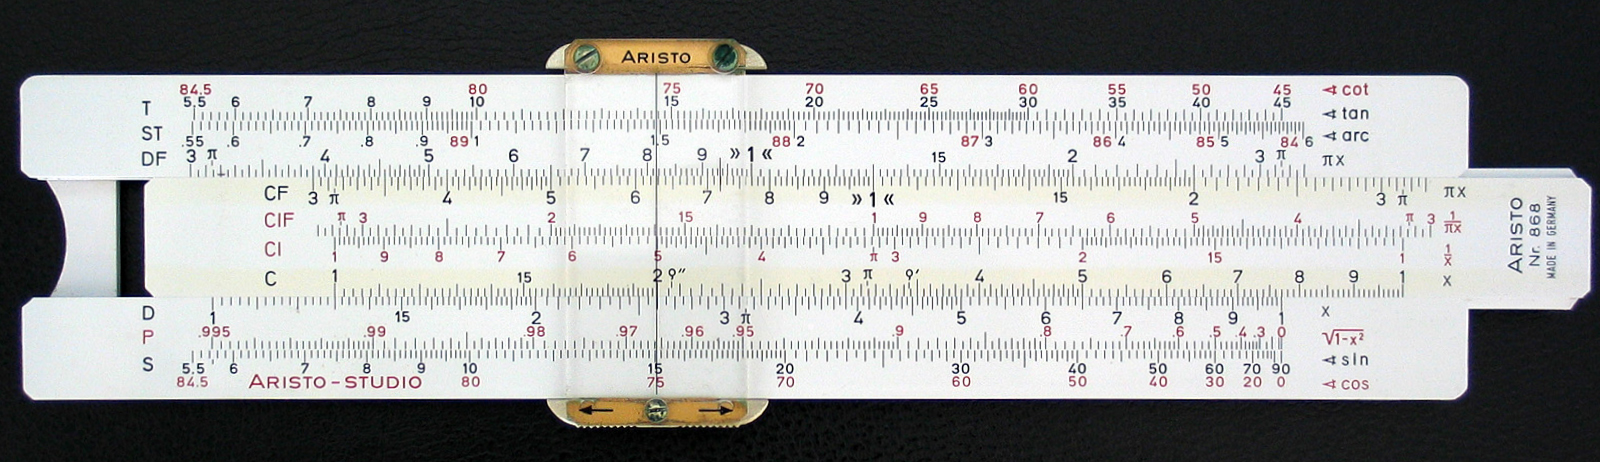
\includegraphics{siber.10}\hss}}{Кружни декадни логаритмар.}
\hbox to 0pt{\hss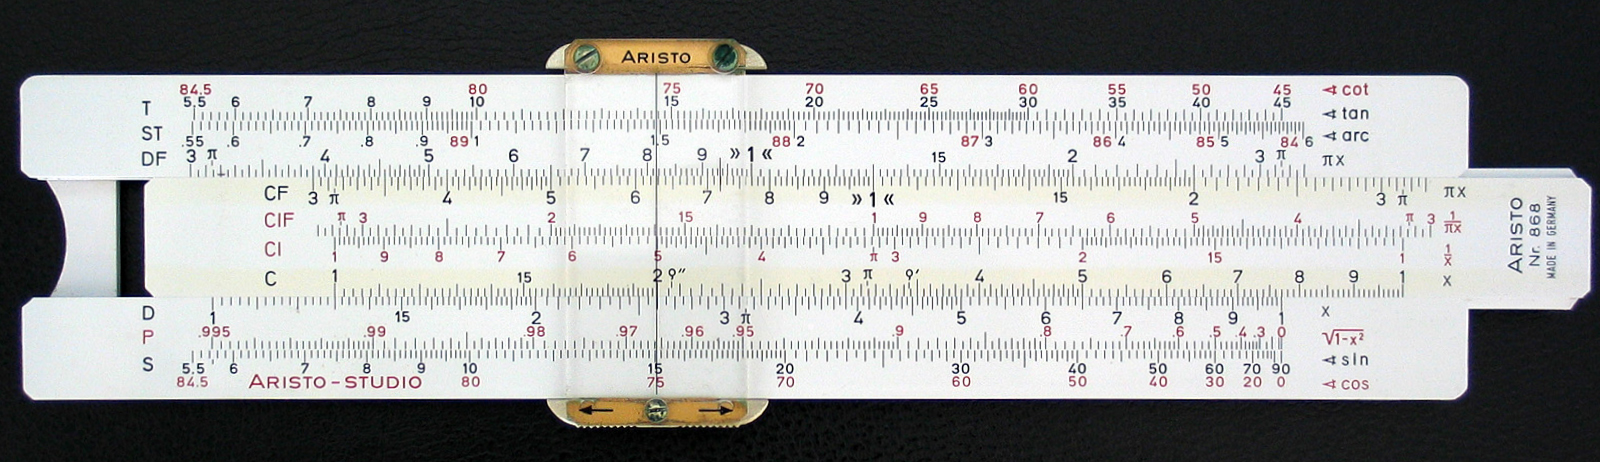
\includegraphics{siber.10}\hss}
$$

\iftrue
\newpage

\pagecolor{karton}
\thispagestyle{empty}
\leavevmode\hbox{}

\vfill

\begin{center}
\def\QR{\GitHubRaw log-cyr.pdf}
\qrcode{\QR}\index{QR}
\end{center}

\fi

% \end{alphasection}

\end{document}
% F22DN-8M46J-2328G-DTK9B-F9CKG

Two-Factor Authentication Backup Codes
Workspace: Instant Win Gaming - https://instantwingaming.slack.com/
Email: undefined

416987660
382212281
363820842
225416942
839219873
815236988
384609006
453026501
992989836
260832280